\documentclass{beamer}[10]

\usepackage{graphicx}
\usepackage{xcolor}
\usepackage{tabto}
%\usepackage{beamerthemesplit}
\usepackage{tikz}
\usepackage{cancel}
\usepackage{verbatim}
\usepackage{fancybox}
\usepackage{enumerate}
\usepackage{amsmath,amssymb,amsthm,textcomp,mathtools}
\usepackage[super]{nth}
\usepackage[amssymb]{SIunits}
\usepackage{booktabs}
\usepackage{cancel}
\usepackage{bm}
\usepackage[utf8]{inputenc}
\usepackage{tabularx}
\usepackage{ragged2e}
\newcolumntype{Y}{ >{\RaggedRight\arraybackslash}X}
\usetikzlibrary{arrows,shapes}
\newcommand\T{\rule{0pt}{2.6ex}}
\newcommand\B{\rule[-1.2ex]{0pt}{0pt}}
\definecolor{UUcrimson}{RGB}{204,0,0}
\mode<presentation>
{ \usetheme{default}
  \usecolortheme[named=UUcrimson]{structure}
  \useinnertheme{circles}
  \setbeamercovered{transparent}
  \setbeamertemplate{blocks}[rounded]
  \usefonttheme[onlymath]{serif}
  \setbeamertemplate{navigation symbols}{}
  \setbeamertemplate{footline}[page number]
  \setbeamertemplate{navigation symbols}{}
  \setbeamercolor{section in toc}{fg=black,bg=white}
  \setbeamercolor{alerted text}{fg=UUcrimson!80!gray}
  \setbeamercolor*{palette primary}{fg=white,bg=UUcrimson}
  \setbeamercolor*{palette secondary}{fg=UUcrimson!70!black,bg=gray!15!white}
  \setbeamercolor*{palette tertiary}{bg=UUcrimson!80!black,fg=gray!10!white}
  \setbeamercolor*{palette quaternary}{fg=UUcrimson,bg=gray!5!white}
  \setbeamercolor*{palette sidebar primary}{fg=UUcrimson!10!black}
  \setbeamercolor*{palette sidebar secondary}{fg=white}
  \setbeamercolor*{palette sidebar tertiary}{fg=UUcrimson!50!black}
  \setbeamercolor*{palette sidebar quaternary}{fg=gray!10!white}
  \setbeamercolor{titlelike}{parent=palette primary,fg=white}
  \setbeamercolor{frametitle}{bg=UUcrimson}
  \setbeamercolor{frametitle right}{bg=UUcrimson}
  \setbeamercolor*{separation line}{}
  \setbeamercolor*{fine separation line}{}
}

\usetikzlibrary{backgrounds}
\makeatletter
\tikzstyle{every picture}+=[remember picture]
\tikzset{%
  fancy quotes/.style={
    text width=\fq@width pt,
    align=justify,
    inner sep=1em,
    anchor=north west,
    minimum width=\linewidth,
    font=\itshape
  },
  fancy quotes width/.initial={.8\linewidth},
  fancy quotes marks/.style={
    scale=8,
    text=white,
    inner sep=0pt,
  },
  fancy quotes opening/.style={
    fancy quotes marks,
  },
  fancy quotes closing/.style={
    fancy quotes marks,
  },
  fancy quotes background/.style={
    show background rectangle,
    inner frame xsep=0pt,
    background rectangle/.style={
      fill=gray!25,
      rounded corners,
    },
  }
}
\newenvironment{fancyquotes}[1][]{%
\noindent
\tikzpicture[fancy quotes background]
\node[fancy quotes opening,anchor=north west] (fq@ul) at (0,0) {``};
\tikz@scan@one@point\pgfutil@firstofone(fq@ul.east)
\pgfmathsetmacro{\fq@width}{\linewidth - 2*\pgf@x}
\node[fancy quotes,#1] (fq@txt) at (fq@ul.north west) \bgroup}
{\egroup;
\node[overlay,fancy quotes closing,anchor=east] at (fq@txt.south east) {''};
\endtikzpicture}
\makeatother

\usepackage{scalerel}[2014/03/10]
\usepackage{stackengine}
\usepackage{empheq}
\newcommand*\widefbox[1]{\fbox{\hspace{0.5em}#1\hspace{0.5em}}}

\newcommand\reallywidetilde[1]{\ThisStyle{%
  \setbox0=\hbox{$\SavedStyle#1$}%
  \stackengine{-.1\LMpt}{$\SavedStyle#1$}{%
    \stretchto{\scaleto{\SavedStyle\mkern.2mu\sim}{.5467\wd0}}{.4\ht0}%
%    .2mu is the kern imbalance when clipping white space
%    .5467++++ is \ht/[kerned \wd] aspect ratio for \sim glyph
  }{O}{c}{F}{T}{S}%
}}
\usepackage{media9}

\logo{
\includegraphics[width=0.75cm]{logo.jpg}}
\author[Gibbs]{Dr. Jeremy A. Gibbs}
\institute{Department of Mechanical Engineering\\University of Utah}
\date{Fall 2016}
\title{LES of Turbulent Flows: Lecture 6}

\begin{document}

%----------------------------------------------------------------------------------------
%	TITLE & TOC SLIDES
%----------------------------------------------------------------------------------------

\begin{frame} 
  \titlepage
\end{frame}

%------------------------------------------------

\begin{frame}
\frametitle{Overview}
\tableofcontents
\end{frame}

%------------------------------------------------
\section{Recap of filters} %
%------------------------------------------------
\begin{frame}{Decomposition of turbulence for real filters}

\begin{itemize}
	\item The LES filter can be used to decompose the velocity field into resolved and subfilter scale (SFS) components:
	$$\underbrace{\phi(\vec{x},t)}_{\text{total}} = \underbrace{\tilde \phi (\vec{x},t)}_{\text{resolved}} + \underbrace{\phi^{\prime}(\vec{x},t)}_{\text{subfilter}}$$
	\item We can use our filtered DNS fields to look at how the choice of our filter kernel affects this separation in wavespace.
\end{itemize}
\end{frame}

%------------------------------------------------

\begin{frame}{Decomposition of turbulence for real filters}
\begin{figure}
	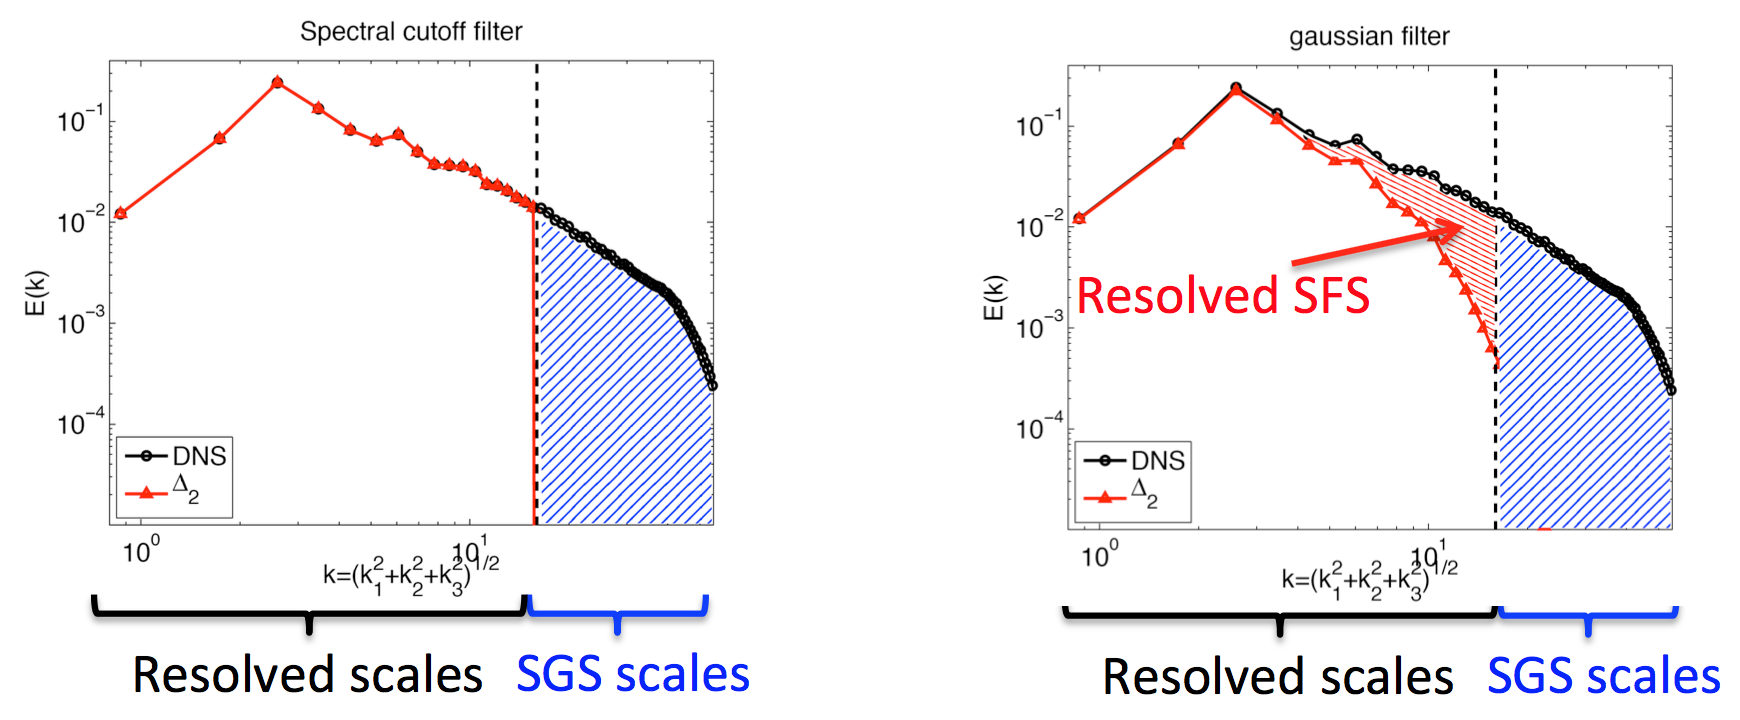
\includegraphics[width=1\textwidth]{filter_decomp.png}
\end{figure}
\begin{itemize}
	\item The Gaussian (or box) filter does not have as compact of support in wavespace as the cutoff filter.
	\item This results in attenuation of energy at scales larger than the filter scale.
	\item The scales affected by the attenuation are referred to as \textit{resolved SFSs}.
\end{itemize}
\end{frame}

%------------------------------------------------
\section{Deriving the incompressible equations of motion} %
%------------------------------------------------
\begin{frame}{Deriving the incompressible equations of motion}

\begin{itemize}
	\item We want to apply the filters to the N-S equations of motion.
	\item First, let's start with the fully compressible form of the equations of motion and derive the incompressible counterparts.
	\item Next, we will apply the filtering operation to the incompressible equations of motion.
	\item Lastly, we will relate the final forms of the equations to the conceptual idea of LES.
\end{itemize}
\end{frame}

%------------------------------------------------

\begin{frame}{Conservation of mass}

We start with the full equation for the conservation of mass:
$$\frac{\partial \rho}{\partial t} + \frac{\partial (\rho u_i)}{\partial x_i} = 0$$
We apply the incompressibility condition -- that a fluid parcel's density is constant ($\rho = \rho_o$):
$$\cancelto{0}{\frac{\partial \rho_o}{\partial t}} + \cancel{\rho_o}\frac{\partial u_i}{\partial x_i} = 0$$
Finally, we divide by $\rho_o$ to arrive at the conservation of mass equation for incompressible flows:
$$\boxed{\frac{\partial u_i}{\partial x_i} = 0}$$
\end{frame}

%------------------------------------------------

\begin{frame}{Conservation of momentum}

We start with the full equation for the conservation of momentum:
$$\frac{\partial (\rho u_i)}{\partial t} + \frac{\partial (\rho u_i u_j)}{\partial x_j} = \frac{\partial}{\partial x_j}\left[ 2\mu S_{ij} - \frac{2}{3}\mu \delta_{ij} \frac{\partial u_i}{\partial x_i}\right] - \frac{\partial p}{\partial x_j} + F_i$$
Apply the incompressibility condition:
$$\rho_o\frac{\partial u_i}{\partial t} + \rho_o\frac{\partial (u_i u_j)}{\partial x_j} = \frac{\partial}{\partial x_j}\left[ 2\mu S_{ij} - \frac{2}{3}\mu \delta_{ij} \frac{\partial u_i}{\partial x_i}\right] - \frac{\partial p}{\partial x_j} + F_i$$
Divide by $\rho_o$:
$$\frac{\partial u_i}{\partial t} + \frac{\partial (u_i u_j)}{\partial x_j} = \frac{\mu}{\rho_o} \frac{\partial}{\partial x_j}\left[ 2 S_{ij} - \frac{2}{3}\mu \delta_{ij} \frac{\partial u_i}{\partial x_i}\right] - \frac{1}{\rho_o}\frac{\partial p}{\partial x_j} + F_i$$
\end{frame}

%------------------------------------------------

\begin{frame}{Conservation of momentum}

Recall that 
$$\nu = \mu/\rho_o \qquad \mbox{and} \qquad S_{ij} = \frac{1}{2}\left(\frac{\partial u_i}{\partial x_j} + \frac{\partial u_j}{\partial x_i}\right)$$
To arrive at:
$$\frac{\partial u_i}{\partial t} + \frac{\partial (u_i u_j)}{\partial x_j} = \nu \frac{\partial}{\partial x_j}\left[\frac{\partial u_i}{\partial x_j} + \frac{\partial u_j}{\partial x_i} - \frac{2}{3}\mu \delta_{ij} \cancelto{0}{\frac{\partial u_i}{\partial x_i}} \right] - \frac{1}{\rho_o}\frac{\partial p}{\partial x_j} + F_i$$
And we can apply the incompressible mass conservation equation and distribute the $\partial/\partial x_j$ in the first term on the right side:
$$\frac{\partial u_i}{\partial t} + \frac{\partial (u_i u_j)}{\partial x_j} = \nu \left[\frac{\partial^2 u_i}{\partial x_j^2} + \frac{\partial^2 u_i}{\partial x_i\partial x_j} \right] - \frac{1}{\rho_o}\frac{\partial p}{\partial x_j} + F_i$$
\end{frame}


%------------------------------------------------

\begin{frame}{Conservation of momentum}

We can rearrange and again apply the mass continuity equation:
$$\frac{\partial u_i}{\partial t} + \frac{\partial (u_i u_j)}{\partial x_j} = \nu \frac{\partial^2 u_i}{\partial x_j^2} + \nu\frac{\partial}{\partial x_j}\cancelto{0}{\left(\frac{\partial u_i}{\partial x_i}\right)} - \frac{1}{\rho_o}\frac{\partial p}{\partial x_j} + F_i$$
and we arrive at the conservation of momentum equation for incompressible flows:
$$\boxed{\frac{\partial u_i}{\partial t} + \frac{\partial (u_i u_j)}{\partial x_j} = - \frac{1}{\rho_o}\frac{\partial p}{\partial x_j} + \nu \frac{\partial^2 u_i}{\partial x_j^2} + F_i}$$
\end{frame}

%------------------------------------------------

\begin{frame}{Conservation of a general scalar}

We start with the full equation for the conservation of momentum:
$$\frac{\partial (\rho \theta)}{\partial t} + \frac{\partial (\rho u_i \theta)}{\partial x_j} = \frac{\partial}{\partial x_j}\left[ \nu_{\theta} \rho \frac{\partial \theta}{\partial x_j}\right] + Q$$
Apply the incompressibility condition:
$$\cancel{\rho_o} \frac{\partial \theta}{\partial t} + \cancel{\rho_o} \frac{\partial (u_i \theta)}{\partial x_j} = \nu_{\theta} \cancel{\rho_o}\frac{\partial}{\partial x_j}\left[\frac{\partial \theta}{\partial x_j}\right] + Q$$
Divide by $\rho_o$ and we arrive at the conservation of a general scalar equation for incompressible flows:
$$\boxed{\frac{\partial \theta}{\partial t} + \frac{\partial (u_i \theta)}{\partial x_j} = \nu_{\theta}\frac{\partial^2 \theta}{\partial x_j^2} + Q}$$
\end{frame}

%------------------------------------------------
\section{Non-dimensional incompressible equations of motion} %
%------------------------------------------------

\begin{frame}{Non-dimensional incompressible equations of motion}
Recall that we can non-dimensionalize these equations by using representative scales, $U$ and $\ell$:
\begin{align*}
u_i^* &= \frac{u_i}{U}\\
x_i^* &= \frac{x_i}{\ell}\\
p^* &= \frac{p}{\rho U^2}\\
t^* &= \frac{t U}{\ell}\\
\theta^* &= \frac{\theta}{\theta_o}
\end{align*}
where the $^*$ denotes a non-dimensionalized term.
\end{frame}

%------------------------------------------------

\begin{frame}{Non-dimensional conservation of mass}

Start with the incompressible conservation of mass and apply the non-dimensional relationships:
$$\frac{\partial u_i}{\partial x_i} = \frac{\partial (u_i^* U)}{\partial (x_i^* \ell)} = \cancel{\frac{U}{\ell}}\frac{\partial u_i^*}{\partial x_i^*} = 0$$
divide by $U/\ell$ to arrive at the non-dimensional incompressible conservation of mass:
$$\boxed{\frac{\partial u_i^*}{\partial x_i^*} = 0}$$
\end{frame}

%------------------------------------------------

\begin{frame}{Non-dimensional conservation of momentum}

Start with the incompressible conservation of momentum and apply the non-dimensional relationships:
\begin{gather*}
\frac{\partial u_i}{\partial t} + \frac{\partial (u_i u_j)}{\partial x_j} = - \frac{1}{\rho_o}\frac{\partial p}{\partial x_j} + \nu \frac{\partial^2 u_i}{\partial x_j^2} + F_i\\
\Rightarrow \frac{\partial (u_i^* U^2)}{\partial t^* \ell} + \frac{\partial (u_i^* u_j^* U^2)}{\partial x_j^*\ell} = - \frac{1}{\rho_o}\frac{\partial (p^* \rho_o U^2)}{\partial x_j^* \ell} + \nu \frac{\partial^2 (u_i^* U)}{\partial x_j^{*2}\ell^2} + F_i
\end{gather*}
Recall that Re=$U\ell/\nu \Rightarrow \nu = U\ell/$Re:
$$
\cancel{\frac{U^2}{\ell}}\frac{\partial u_i^*}{\partial t^*} + \cancel{\frac{U^2}{\ell}}\frac{\partial (u_i^* u_j^*)}{\partial x_j^*} = - \cancel{\frac{U^2}{\ell}}\frac{1}{\cancel{\rho_o}}\frac{\partial (p^* \cancel{\rho_o})}{\partial x_j^*} + \cancel{\frac{U^2}{\ell}}\frac{1}{Re} \frac{\partial^2 u_i^*}{\partial x_j^{*2}} + F_i
$$
divide by $U^2/\ell$ to arrive at the non-dimensional incompressible conservation of momentum:
$$\boxed{\frac{\partial u_i^*}{\partial t^*} + \frac{\partial (u_i^* u_j^*)}{\partial x_j^*} = - \frac{\partial p^*}{\partial x_j^*} + \frac{1}{Re} \frac{\partial^2 u_i^*}{\partial x_j^{*2}} + F_i}$$
\end{frame}

%------------------------------------------------

\begin{frame}{Non-dimensional conservation of a general scalar}

Start with the incompressible conservation of a general scalar and apply the non-dimensional relationships:
\begin{gather*}
\frac{\partial \theta}{\partial t} + \frac{\partial (u_i \theta)}{\partial x_j} = \nu_{\theta}\frac{\partial^2 \theta}{\partial x_j^2} + Q\\
\Rightarrow \frac{\partial \theta^* \theta_o U}{\partial t^* \ell} + \frac{\partial (u_i^* \theta^* \theta_o)}{\partial x_j^* \ell} = \nu_{\theta}\frac{\partial^2 \theta^* \theta_o}{\partial x_j^{*2} \ell^2} + Q
\end{gather*}
Recall that Sc$=\nu/\nu_{\theta}\Rightarrow \nu_{\theta}=\nu/$Sc$=U\ell/$(Sc\ Re):
$$
\cancel{\frac{U \theta_o}{\ell}}\frac{\partial \theta^*}{\partial t^*} + \cancel{\frac{U \theta_o}{\ell}}\frac{\partial (u_i^*\theta^*)}{\partial x_j^*} =  \cancel{\frac{U\theta_o}{\ell}}\frac{1}{Sc\ Re} \frac{\partial^2 \theta^*}{\partial x_j^{*2}} + Q
$$
divide by $U\theta_o/\ell$ to arrive at the non-dimensional incompressible conservation of a general scalar:
$$\boxed{\frac{\partial \theta^*}{\partial t^*} + \frac{\partial (u_i^* \theta^*)}{\partial x_j^*} = + \frac{1}{Sc\ Re} \frac{\partial^2 \theta^*}{\partial x_j^{*2}} + Q}$$
\end{frame}

%------------------------------------------------
\section{Filtering the incompressible equations of motion} %
%------------------------------------------------
\begin{frame}{Filtering the incompressible equations of motion}
Next we apply the filter to the non-dimensional incompressible equations of motion, recalling that the filters hold the following properties:
\begin{align*}
\tilde a &= a\\
\widetilde{\phi + \zeta} &= \tilde \phi + \tilde \zeta\\
\widetilde{\frac{\partial \phi}{\partial x}} &= 	\frac{\partial \tilde \phi}{\partial x}
\end{align*}
That is: a constant is unaffected by the filter, the filtered sum of two variables is the sum of the filtered variables, and the filter is commutative for differentiation.

\end{frame}
%------------------------------------------------

\begin{frame}{Filtered conservation of mass}

Start with the non-dimensional incompressible conservation of mass and apply the filter (where the $^*$ notation is dropped for convenience):
\begin{gather*}
\widetilde{\frac{\partial u_i}{\partial x_i} = 0}\\
\widetilde{\frac{\partial u_i}{\partial x_i}} = \tilde 0 \\
\boxed{\frac{\partial \tilde u_i}{\partial x_i} = 0}
\end{gather*}

This is the non-dimensional form of the filtered conservation of mass equation for incompressible flows.
\end{frame}

%------------------------------------------------

\begin{frame}{Filtered conservation of momentum}

Start with the non-dimensional incompressible conservation of momentum and apply the filter (where the $^*$ notation is dropped for convenience):
\begin{gather*}
\widetilde{\frac{\partial u_i}{\partial t} + \frac{\partial (u_i u_j)}{\partial x_j} = - \frac{\partial p}{\partial x_j} + \frac{1}{Re} \frac{\partial^2 u_i}{\partial x_j^{2}} + F_i}\\
\widetilde{\frac{\partial u_i}{\partial t}} + \widetilde{\frac{\partial (u_i u_j)}{\partial x_j}} = \widetilde{- \frac{\partial p}{\partial x_j}} + \widetilde{\frac{1}{Re} \frac{\partial^2 u_i}{\partial x_j^{2}}} + F_i \\
\frac{\partial \tilde u_i}{\partial t} + \frac{\partial (\widetilde{u_i u_j})}{\partial x_j} = - \frac{\partial \tilde p}{\partial x_j} + \frac{1}{Re} \frac{\partial^2 \tilde u_i}{\partial x_j^{2}} + F_i
\end{gather*}
We have a problem because $\widetilde{u_i u_j}$ is the filtered product of two non-filtered variables. We do not have knowledge of these variables and thus the term cannot be solved \textit{a priori}.
\end{frame}

%------------------------------------------------

\begin{frame}{Filtered conservation of momentum}

Following Leonard (1974), we can decompose the unknown term as
$$\widetilde{u_i u_j} = \tilde u_i \tilde u_j + \tau_{ij}^r$$
where $\tau_{ij}^r$ is the subfilter scale (SFS) stress tensor. 
\newline\newline We can substitute this back into the previous equation to arrive at the non-dimensional form of the filtered conservation of momentum equation for incompressible flows:
$$\boxed{\frac{\partial \tilde u_i}{\partial t} + \frac{\partial (\tilde u_i \tilde u_j)}{\partial x_j} = - \frac{\partial \tilde p}{\partial x_j} + \frac{1}{Re} \frac{\partial^2 \tilde u_i}{\partial x_j^{2}} -\frac{\partial \tau_{ij}^r}{\partial x_j}+ F_i}$$
Welcome to the closure problem because $\tau_{ij}^r$ is unknown -- thus the equation is not closed. The SFS stress tensor must be modeled.
\end{frame}

%------------------------------------------------

\begin{frame}{Filtered conservation of a general scalar}

Start with the non-dimensional incompressible conservation of a general scalar and apply the filter (where the $^*$ notation is dropped for convenience):
\begin{gather*}
\widetilde{\frac{\partial \theta}{\partial t} + \frac{\partial (u_i \theta)}{\partial x_j} = + \frac{1}{Sc\ Re} \frac{\partial^2 \theta}{\partial x_j^{2}} + Q}\\
\widetilde{\frac{\partial \theta}{\partial t}} + \widetilde{\frac{\partial (u_i \theta)}{\partial x_j}} = + \widetilde{\frac{1}{Sc\ Re} \frac{\partial^2 \theta}{\partial x_j^{2}}} + Q\\
\frac{\partial \tilde \theta}{\partial t} + \frac{\partial (\widetilde{u_i \theta})}{\partial x_j} = \frac{1}{Sc\ Re} \frac{\partial^2 \tilde \theta}{\partial x_j^{2}} + Q
\end{gather*}
Again, we have a problem because $\widetilde{u_i \theta}$ is the filtered product of two non-filtered variables. We do not have knowledge of these variables and thus the term cannot be solved \textit{a priori}.
\end{frame}

%------------------------------------------------

\begin{frame}{Filtered conservation of a general scalar}

We again decompose the unknown term as
$$\widetilde{u_i \theta} = \tilde u_i \tilde \theta + q_i^r$$
where $q_i^r$ is the SFS flux. 
\newline\newline We can substitute this back into the previous equation to arrive at the non-dimensional form of the filtered conservation of momentum equation for incompressible flows:
$$\boxed{\frac{\partial \tilde \theta}{\partial t} + \frac{\partial (\tilde u_i \tilde \theta)}{\partial x_j} = \frac{1}{Sc\ Re} \frac{\partial^2 \tilde \theta}{\partial x_j^{2}} -\frac{\partial q_i^r}{\partial x_j}+ Q}$$
Similarly, $q_i^r$ is unknown -- thus the equation is not closed. The SFS flux must be modeled.
\end{frame}

%------------------------------------------------

\begin{frame}{LES filtered equations for incompressible flows}
Mass
\begin{itemize}
	\item $\frac{\partial \tilde u_i}{\partial x_i} = 0$
\end{itemize}

Momentum
\begin{itemize}
\item $\frac{\partial \tilde u_i}{\partial t} + \frac{\partial (\tilde u_i \tilde u_j)}{\partial x_j} = - \frac{\partial \tilde p}{\partial x_j} + \frac{1}{Re} \frac{\partial^2 \tilde u_i}{\partial x_j^{2}} -\frac{\partial \tau_{ij}^r}{\partial x_j}+ F_i$
\end{itemize}

Scalar
\begin{itemize}
	\item $\frac{\partial \tilde \theta}{\partial t} + \frac{\partial (\tilde u_i \tilde \theta)}{\partial x_j} = \frac{1}{Sc\ Re} \frac{\partial^2 \tilde \theta}{\partial x_j^{2}} -\frac{\partial q_i^r}{\partial x_j}+ Q$
\end{itemize}

SFS stress
\begin{itemize}
	\item $\tau_{ij}^r = \widetilde{u_i u_j} - \tilde u_i \tilde u_j$
\end{itemize}

SFS flux
\begin{itemize}
	\item $q_{i}^r = \widetilde{u_i \theta} - \tilde u_i \tilde \theta$
\end{itemize}
\end{frame}

%------------------------------------------------

\begin{frame}{Up next, turbulence kinetic energy}

\begin{itemize}
\item We've talked about variance (or energy) when discussing turbulence and filtering.
\item When we examined the application of the LES filter at scale $\Delta$ we saw the effect of the filter on the distribution of energy with scale.
\item A natural way to extend our examination of scale separation and energy is to look at the evolution of the filtered variance or turbulence kinetic energy.
\end{itemize}

\end{frame}

%------------------------------------------------

\end{document}

